\section{Resoconto attività di verifica}

\subsection{Revisione dei requisiti}

\subsubsection{ di processo}

Di seguito sono riassunti i risultati delle attività di \glo{verifica} effettuate sui documenti consegnati nelle varie revisioni di progetto.

\subsubsection{ di prodotto}

Le \glo{metriche} stanziate in questa fase sono quelle che riguardano i documenti.

\paragraph{MDC1 Indice di Gulpease}

La metrica MDC1 Indice di Gulpease è stata realizzata grazie all'utilizzo di script automatici. I risultati dell'analisi effettuata sui principali documenti prodotti vengono riassunti nella seguente tabella:

\begin{table}[H]
		\begin{center}
			\setlength{\aboverulesep}{0pt}
			\setlength{\belowrulesep}{0pt}
			\setlength{\extrarowheight}{.75ex}
			\rowcolors{2}{AzzurroGruppo!10}{white}
			\begin{tabular}{ c C{4cm} C{2cm} C{3cm} }
				\rowcolor{AzzurroGruppo!30} 
				\textbf{Nome documento} & \textbf{Indice di Gulpease} & \textbf{Esito} \\
				\toprule
		Studio di Fattibilità & 67 & ottimo\\
		Norme di Progetto & 68 & ottimo\\
		Analisi dei \ignore{Requisiti} & 81 & ottimo\\
		Piano di Progetto & 82 & ottimo\\
		Piano di qualifica & 76 & ottimo\\
			
		\bottomrule
			\end{tabular}
			\caption{Resoconto metrica MDC1 indice di Gulpease}
		\end{center}
	\end{table}

\paragraph{MDC2 Correttezza ortografica}

La correttezza ortografica è stata valutata tramite un attento controllo da parte dei verificatori e tramite il correttore ortografico aspell.  Ogni documento raggiunge il valore accettabile della metrica MDC2 Correttezza ortografica. 
\newpage{}
\subsection{Revisione di progettazione}
\subsubsection{Cruscotto indice di Gulpease}

Di seguito riportiamo il cruscotto dei valori dell'indice di Gulpease valutato sui documenti da consegnare.

\begin{figure}[H]
    \centering
    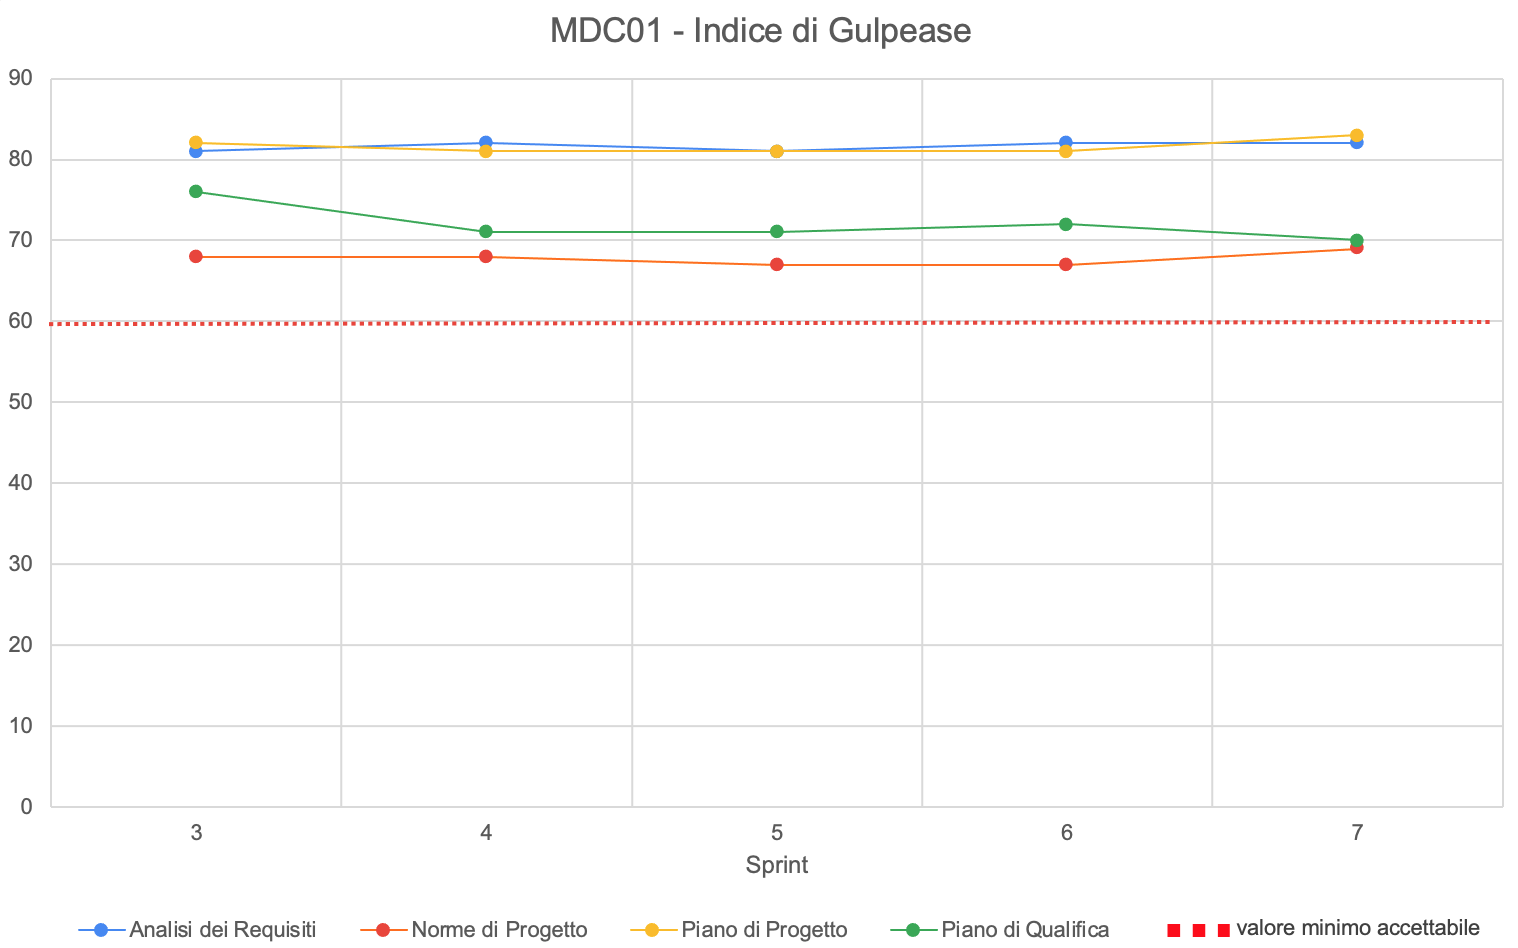
\includegraphics[scale = 0.55]{immagini/GulpeaseRP.png}
    \caption{Cruscotto MDC01, RP}
\end{figure}

\newpage

\subsection{Revisione di qualifica}
\subsubsection{Cruscotto qualità dei documenti}
Di seguito riportiamo i cruscotti dei valori riscontrati delle \glo{metriche} riguardanti i documenti, descritte nel paragrafo \ref{QualitàDoc}.
\subsubsection*{MDC01 - indice di Gulpease}
\begin{figure}[H]
    \centering
    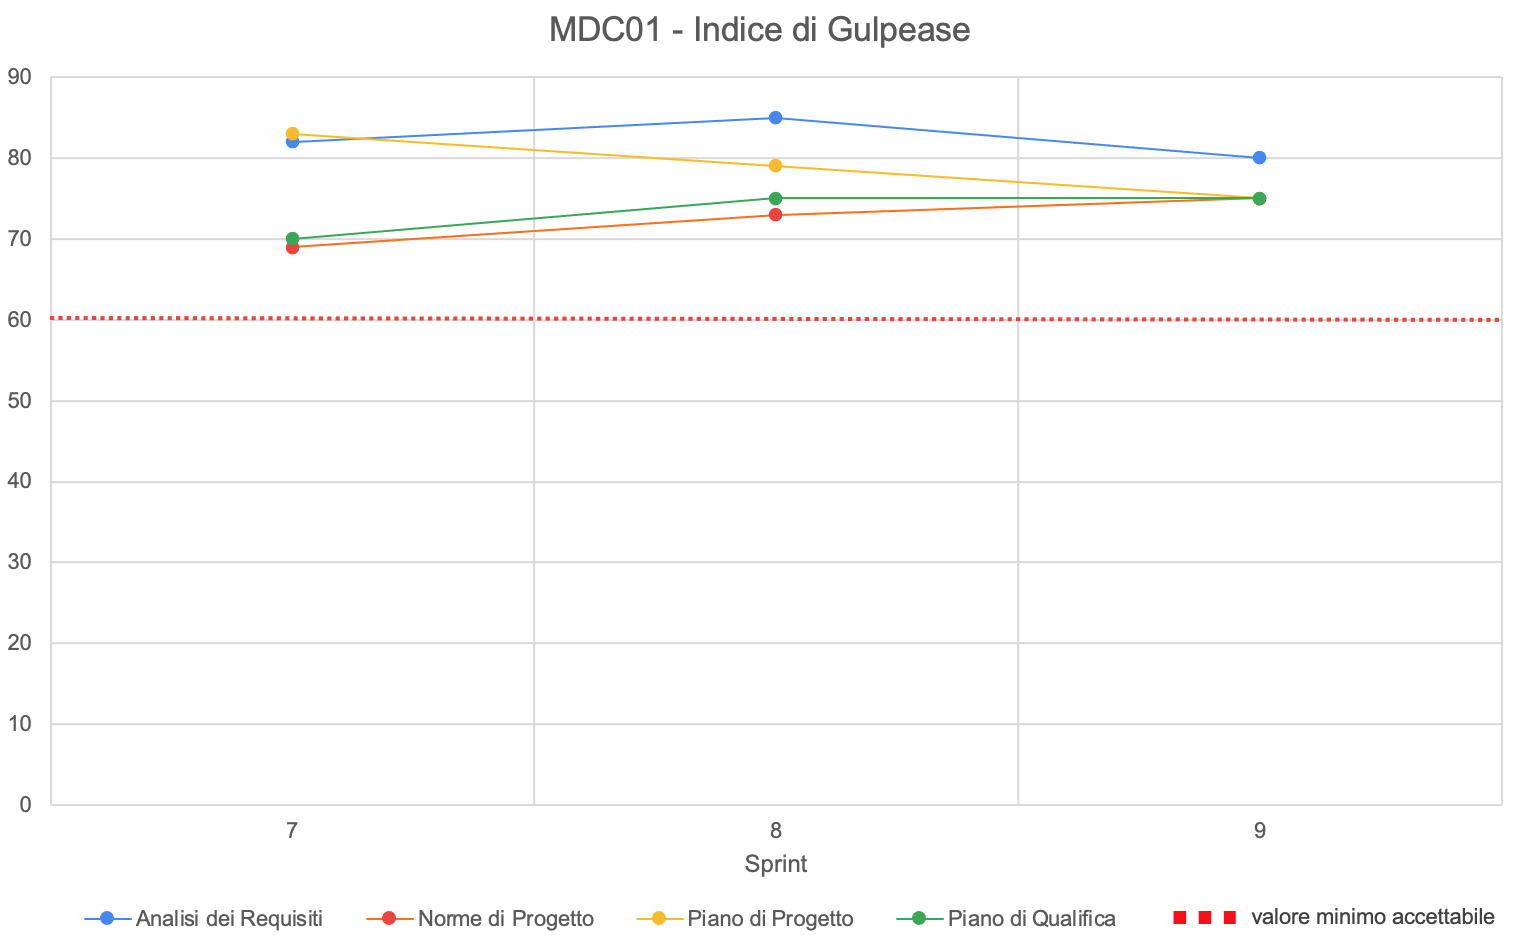
\includegraphics[scale = 0.6]{immagini/GulpeaseRQ.png}
    \caption{Cruscotto MDC01, RQ}
\end{figure}

\subsubsection*{MDC02 - indice di Flesch-Vacca}
\begin{figure}[H]
    \centering
    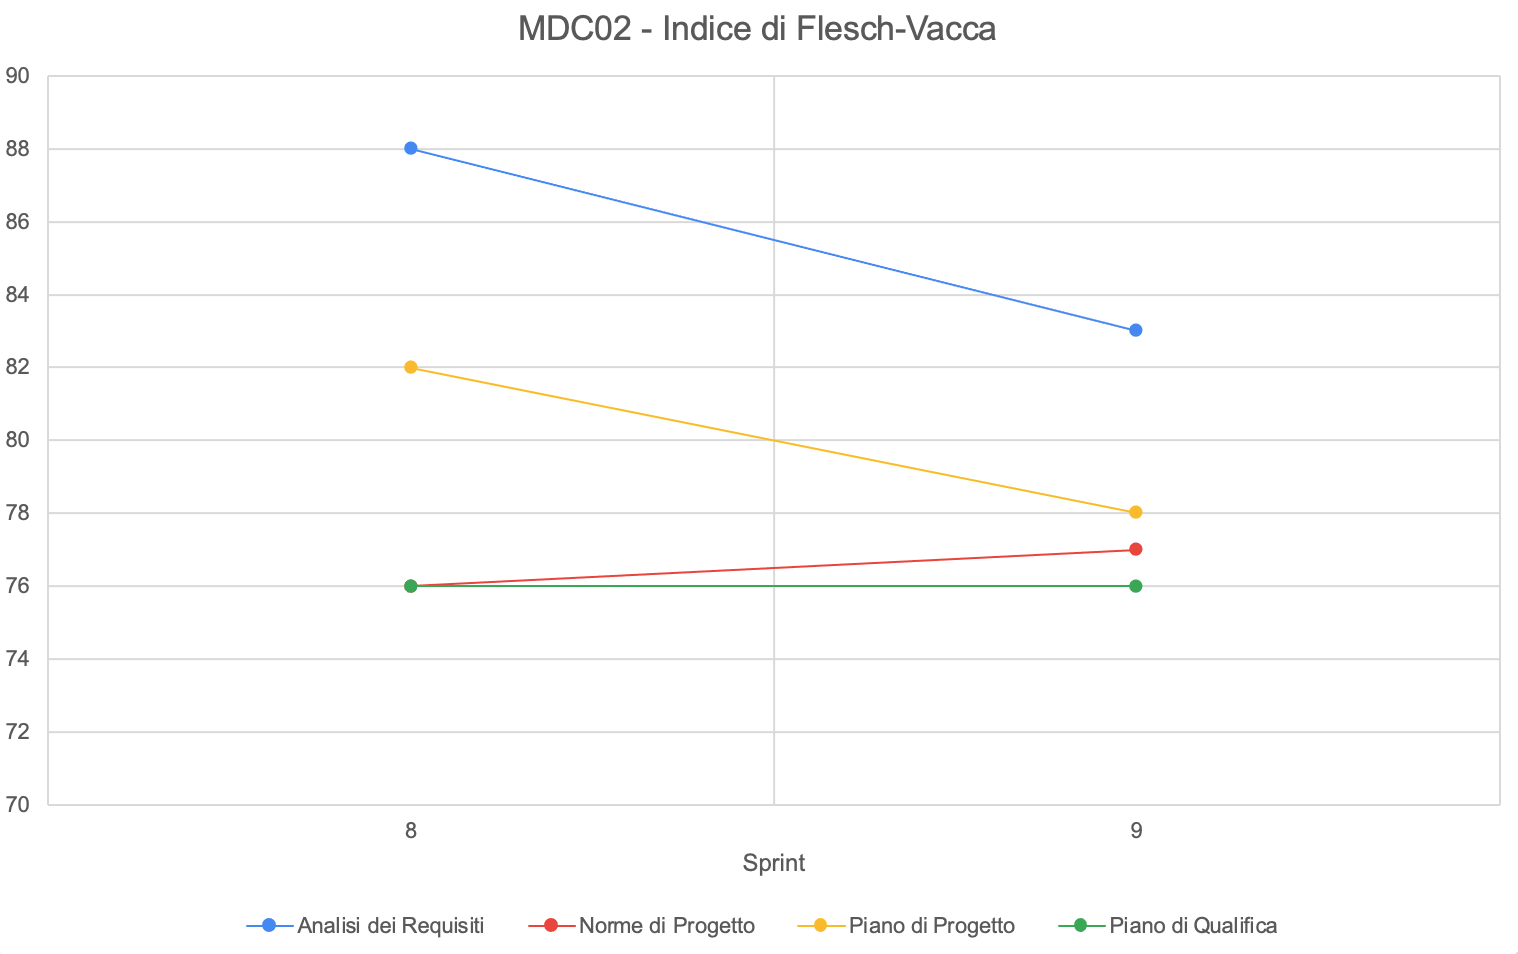
\includegraphics[scale = 0.6]{immagini/fleschRQ.png}
    \caption{Cruscotto MDC02, RQ}
\end{figure}
\newpage
\subsubsection{Cruscotto  qualità del software}
Di seguito riportiamo i cruscotti dei valori riscontrati delle \glo{metriche} riguardanti il codice, descritte nel paragrafo \ref{QualitàSW} . In particolare, i grafici raggruppano le \glo{metriche} appartenenti agli stessi sottoparagrafi.

\subsubsection*{MCD01 - percentuale degli errori corretti}
\begin{figure}[H] 
    \centering
    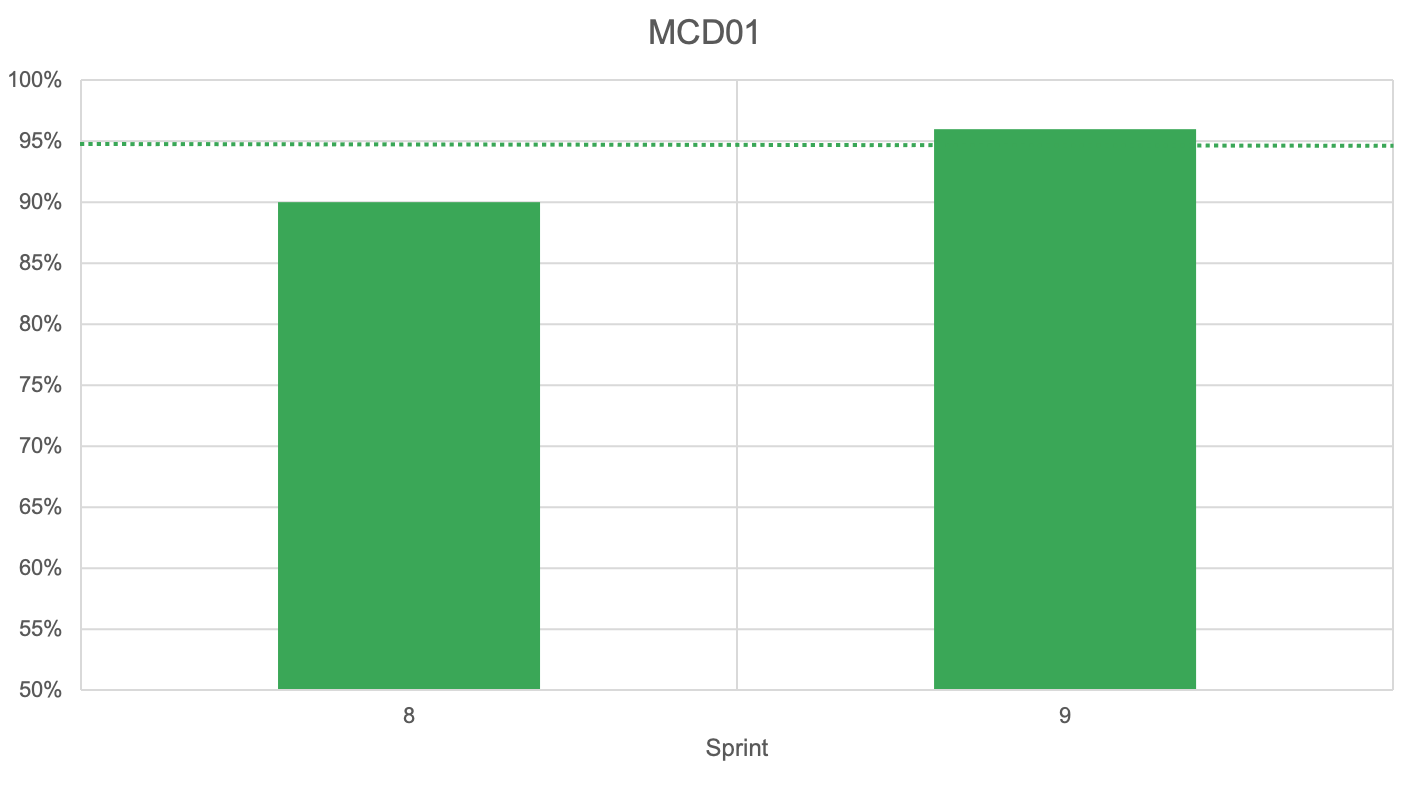
\includegraphics[scale = 0.55]{immagini/MCD01.png}
    \caption{Cruscotto MCD01, RQ}
\end{figure}

\subsubsection*{MCD02 - complessità ciclomatica, MCD06 - lunghezza della riga di codice, MCD07 - brevità dei metodi}
\begin{figure}[H] 
    \centering
    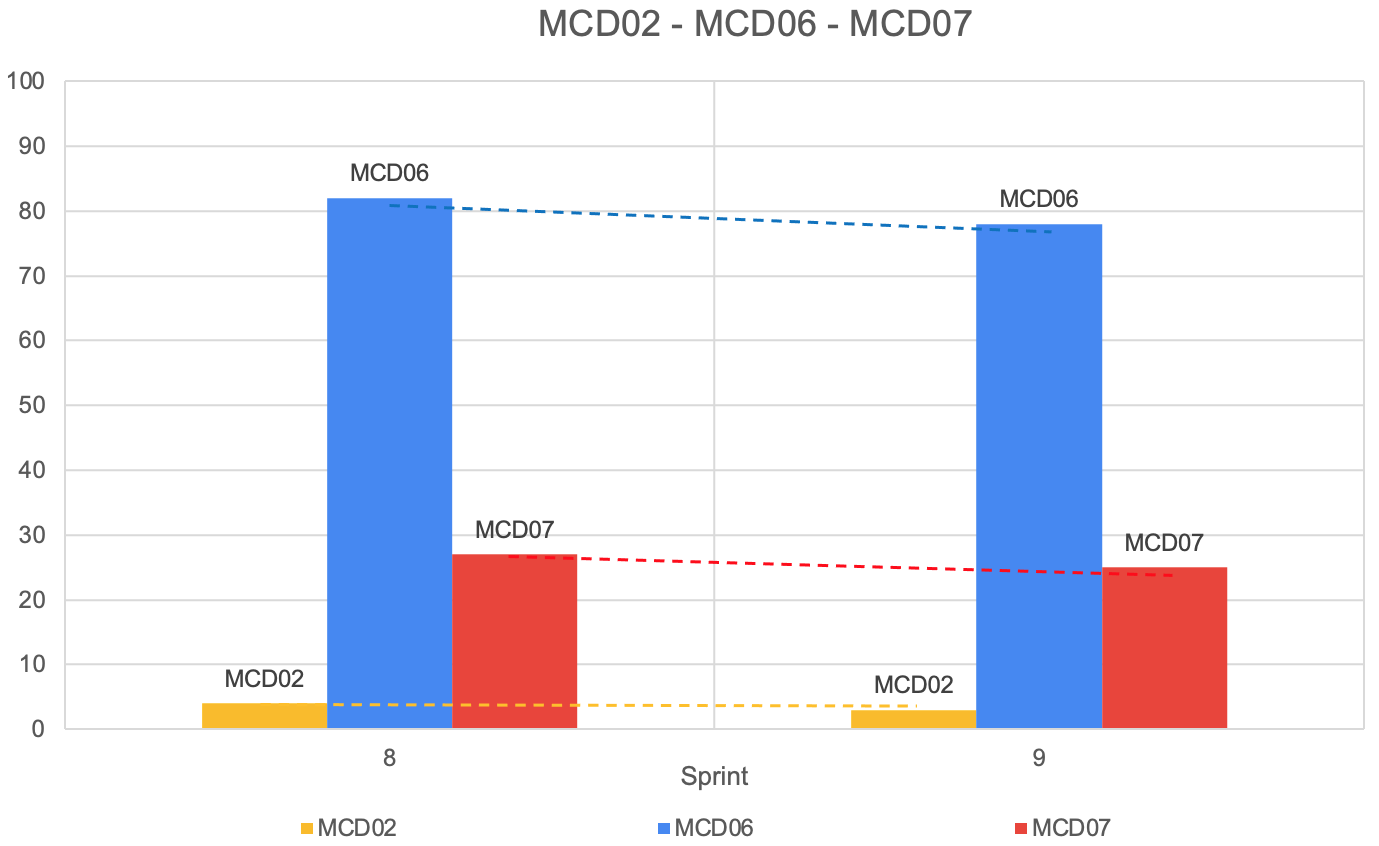
\includegraphics[scale = 0.55]{immagini/MCD02-06-07.png}
    \caption{Cruscotto MCD02, MCD06, MCD07, RQ}
\end{figure}

\subsubsection*{MCD03 - variabili non utilizzate, MCD04 - rapporto linee di codice e linee commentate}
\begin{figure}[H] 
    \centering
    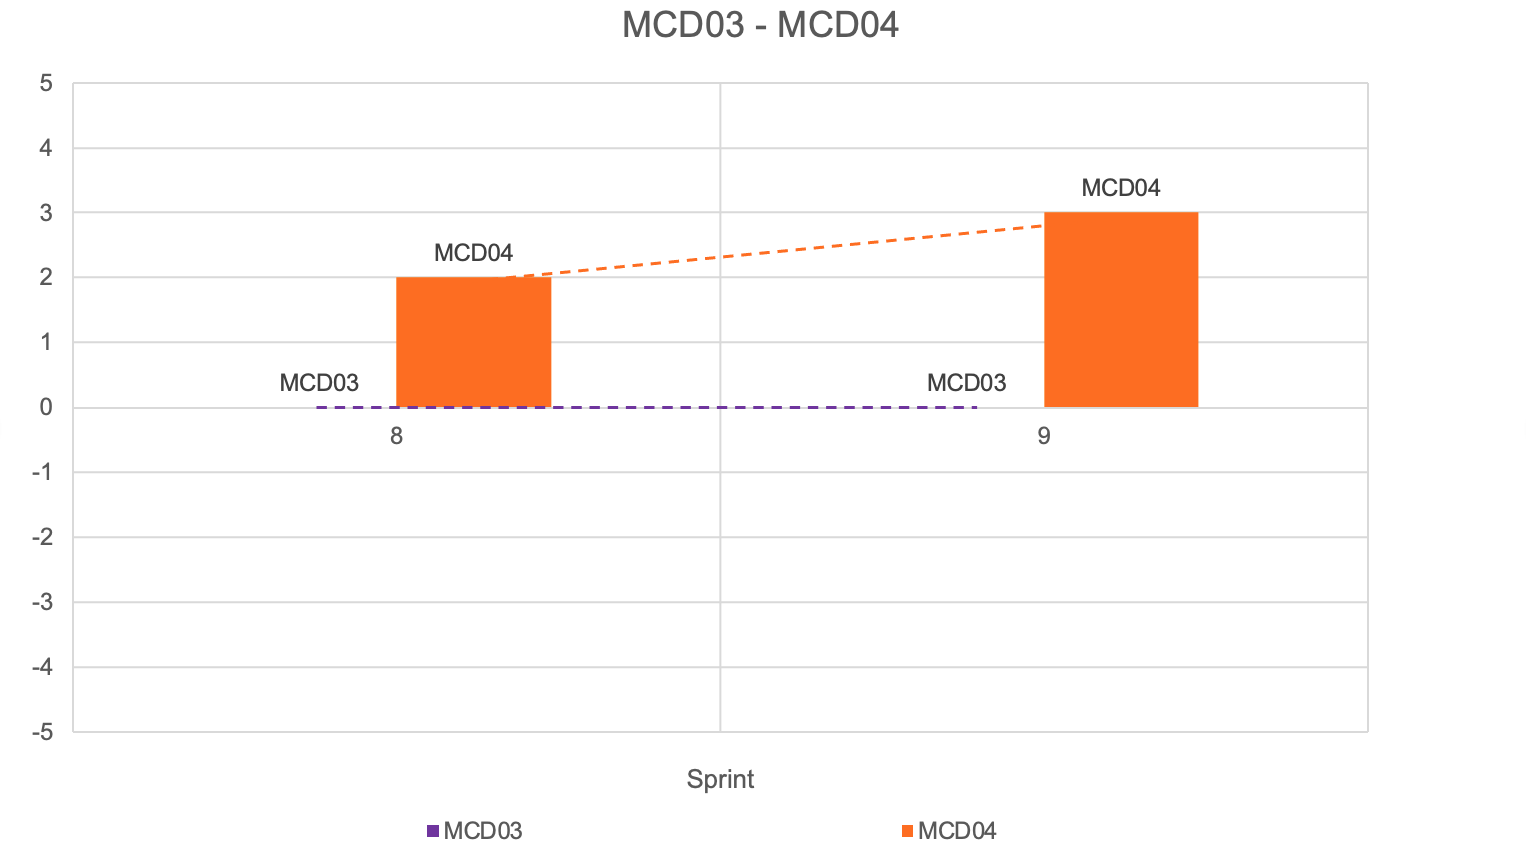
\includegraphics[scale = 0.6]{immagini/MCD03-04.png}
    \caption{Cruscotto MCD03, MCD04, RQ}
\end{figure}

\subsubsection*{MCD05 - code coverage}
\begin{figure}[H] 
    \centering
    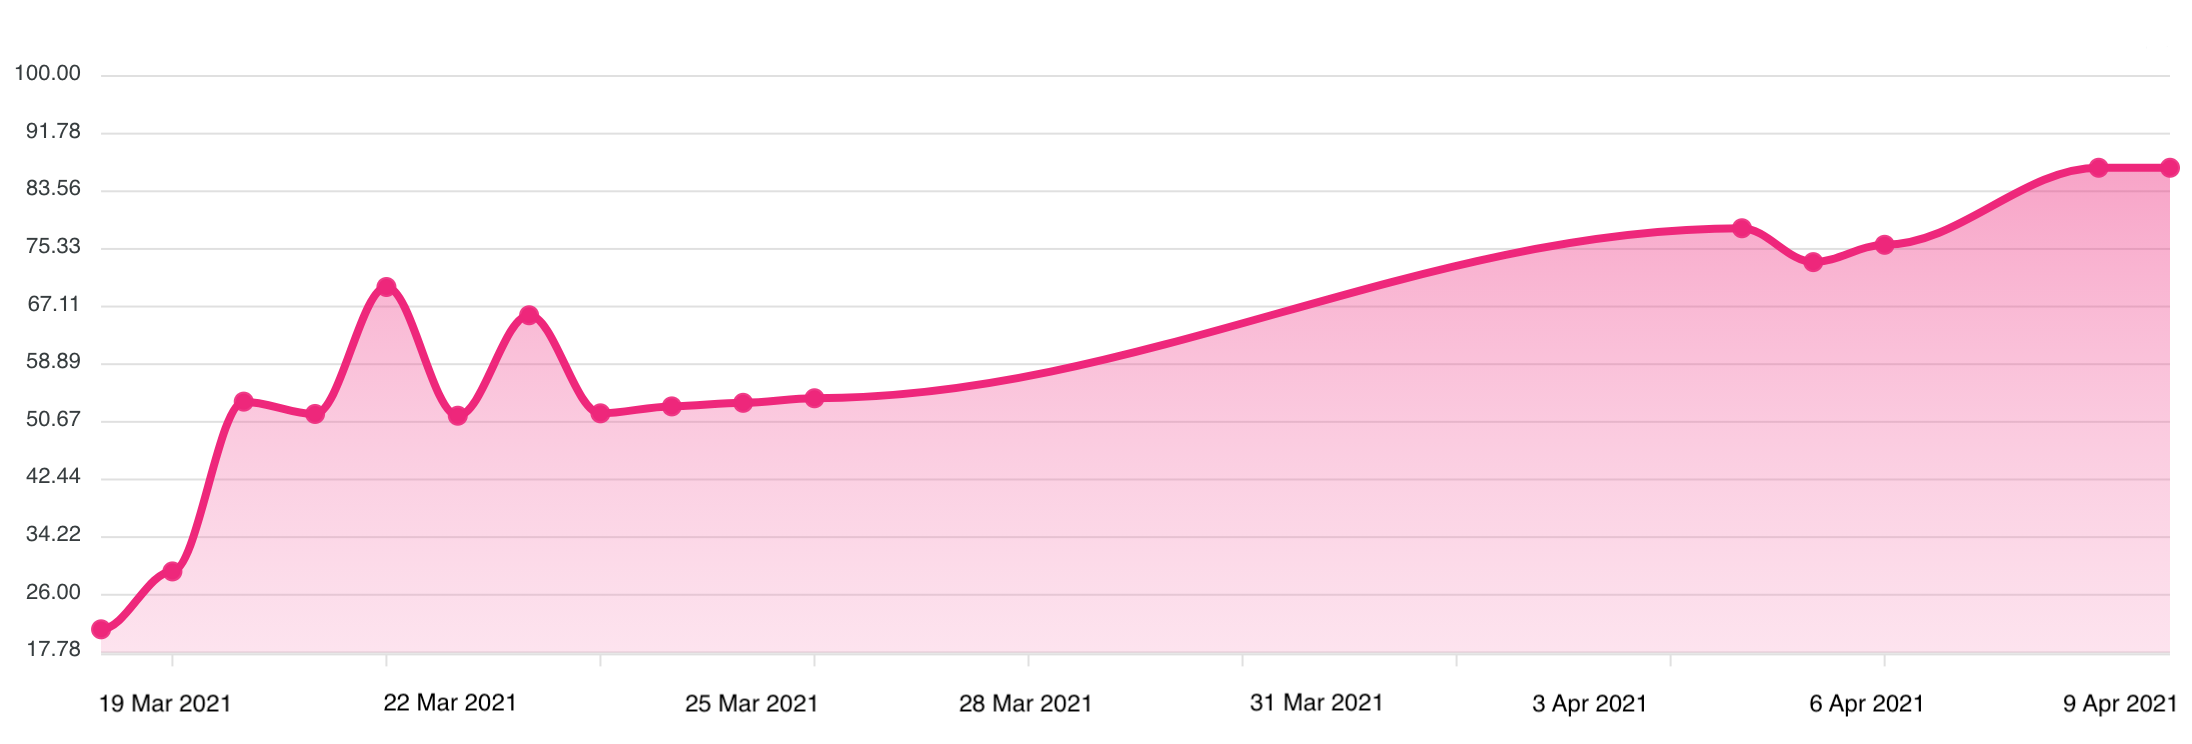
\includegraphics[scale = 0.4]{immagini/MCD05.png}
    \caption{Cruscotto MCD05, RQ}
\end{figure}

\newpage

\subsection{Revisione di accettazione}
\subsubsection{Cruscotto qualità del prodotto}
Di seguito riportiamo i cruscotti dei valori riscontrati delle \glo{metriche} riguardanti il prodotto, descritte nel paragrafo \ref{QProcesso} .  In particolare, le metriche sono raggruppate in base al tipo, come normato nel documento \NdP{}.
\subsubsection*{MCD08 - accoppiamento tra oggetti, MCD09 - numero parametri per metodo, MCD10 -livello di annidamento }

\begin{figure}[H] 
    \centering
    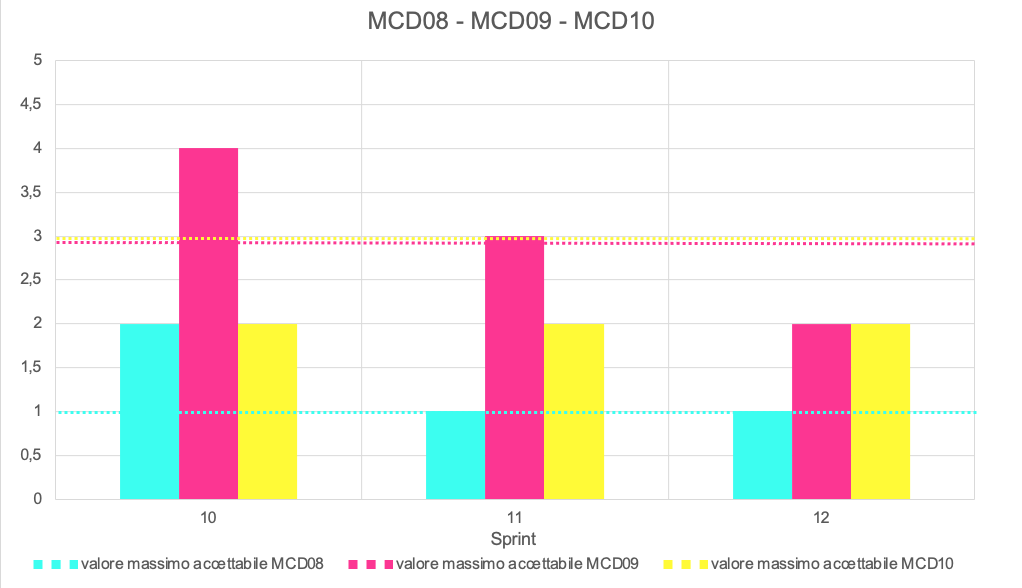
\includegraphics[scale = 0.8]{immagini/ImmRA/MCD080910.png}
    \caption{Cruscotto MCD08-MCD09-MCD10, RA}
\end{figure}

\subsubsection*{MPR01 - variazione schedule, MPR02 - variazione budget}

\begin{figure}[H] 
    \centering
    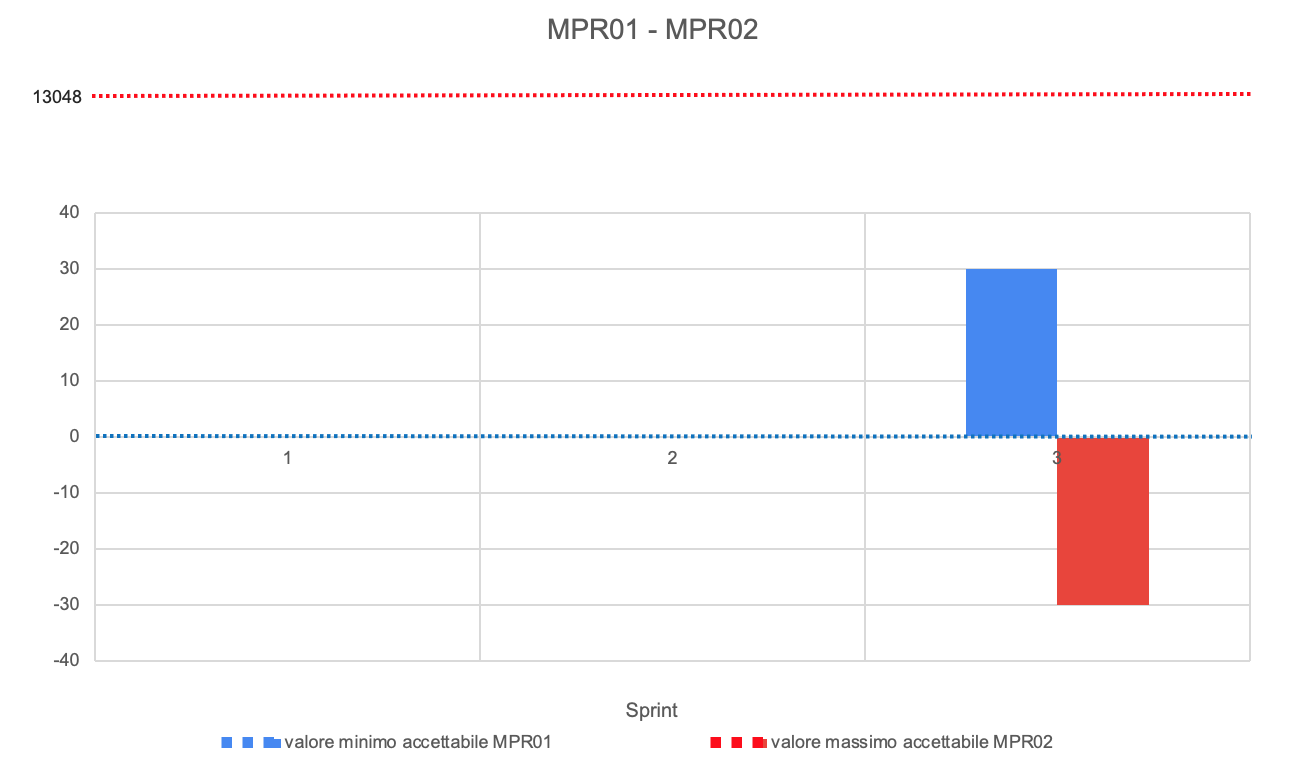
\includegraphics[scale = 0.6]{immagini/ImmRA/MPR0102.png}
    \caption{Cruscotto MPR01-MPR02-, RA}
\end{figure}

\subsubsection*{MPR05 - costo effettivo del lavoro realizzato, MPR06 - costo pianificato del lavoro da realizzare}

\begin{figure}[H] 
    \centering
    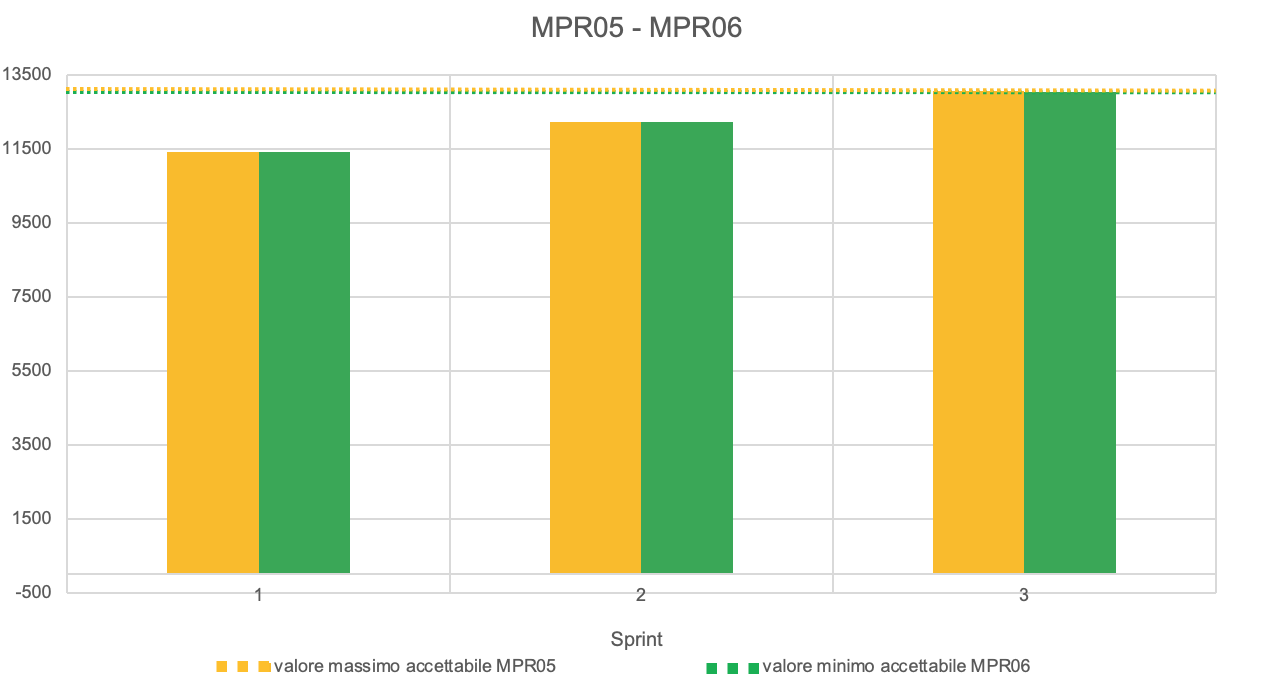
\includegraphics[scale = 0.7]{immagini/ImmRA/MPR0506.png}
    \caption{Cruscotto MPR05-MPR06-, RA}
\end{figure}

\subsubsection{Cruscotto qualità dei documenti}
\subsubsection*{MDC01 - indice di Gulpease}

\begin{figure}[H] 
    \centering
    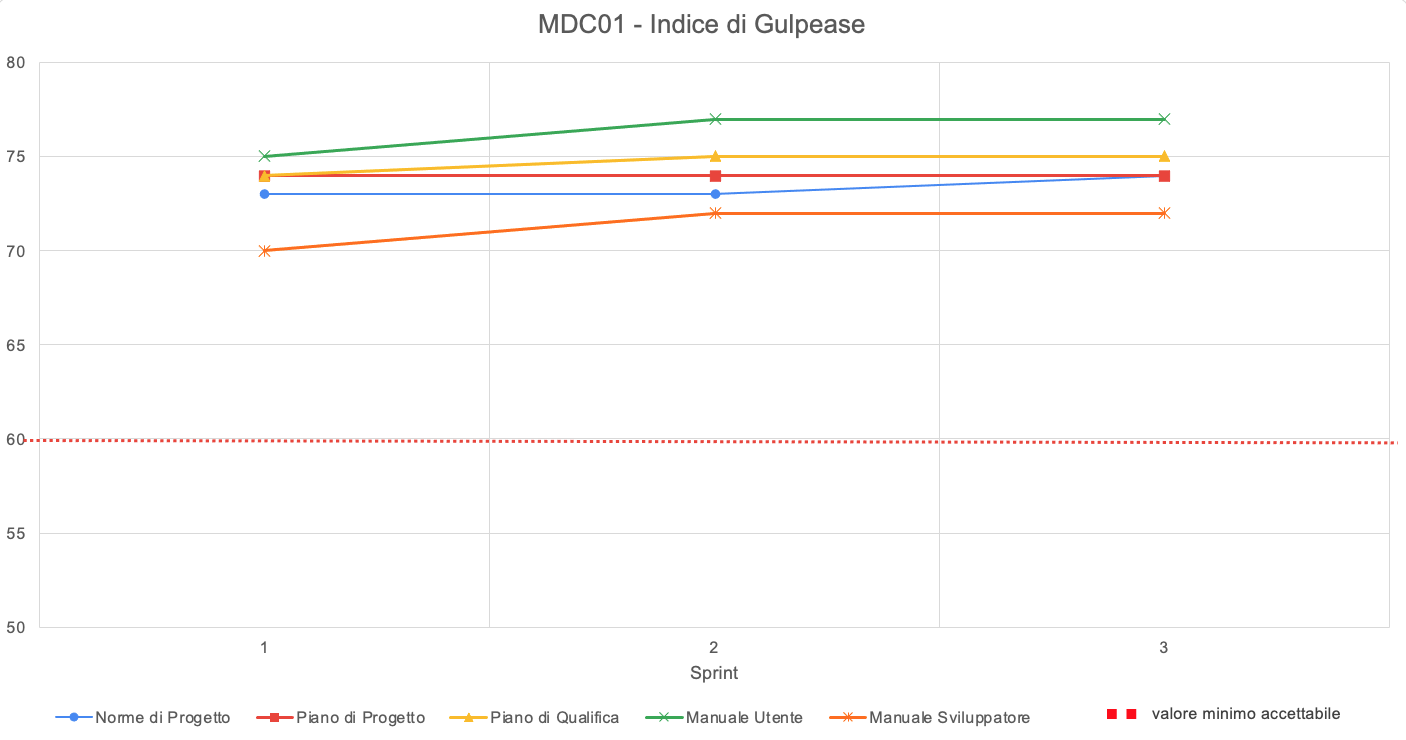
\includegraphics[scale = 0.6]{immagini/ImmRA/MDC01.png}
    \caption{Cruscotto MDC01, RA}
\end{figure}

\subsubsection*{MDC02 - indice di Flesch-Vacca}

\begin{figure}[H] 
    \centering
    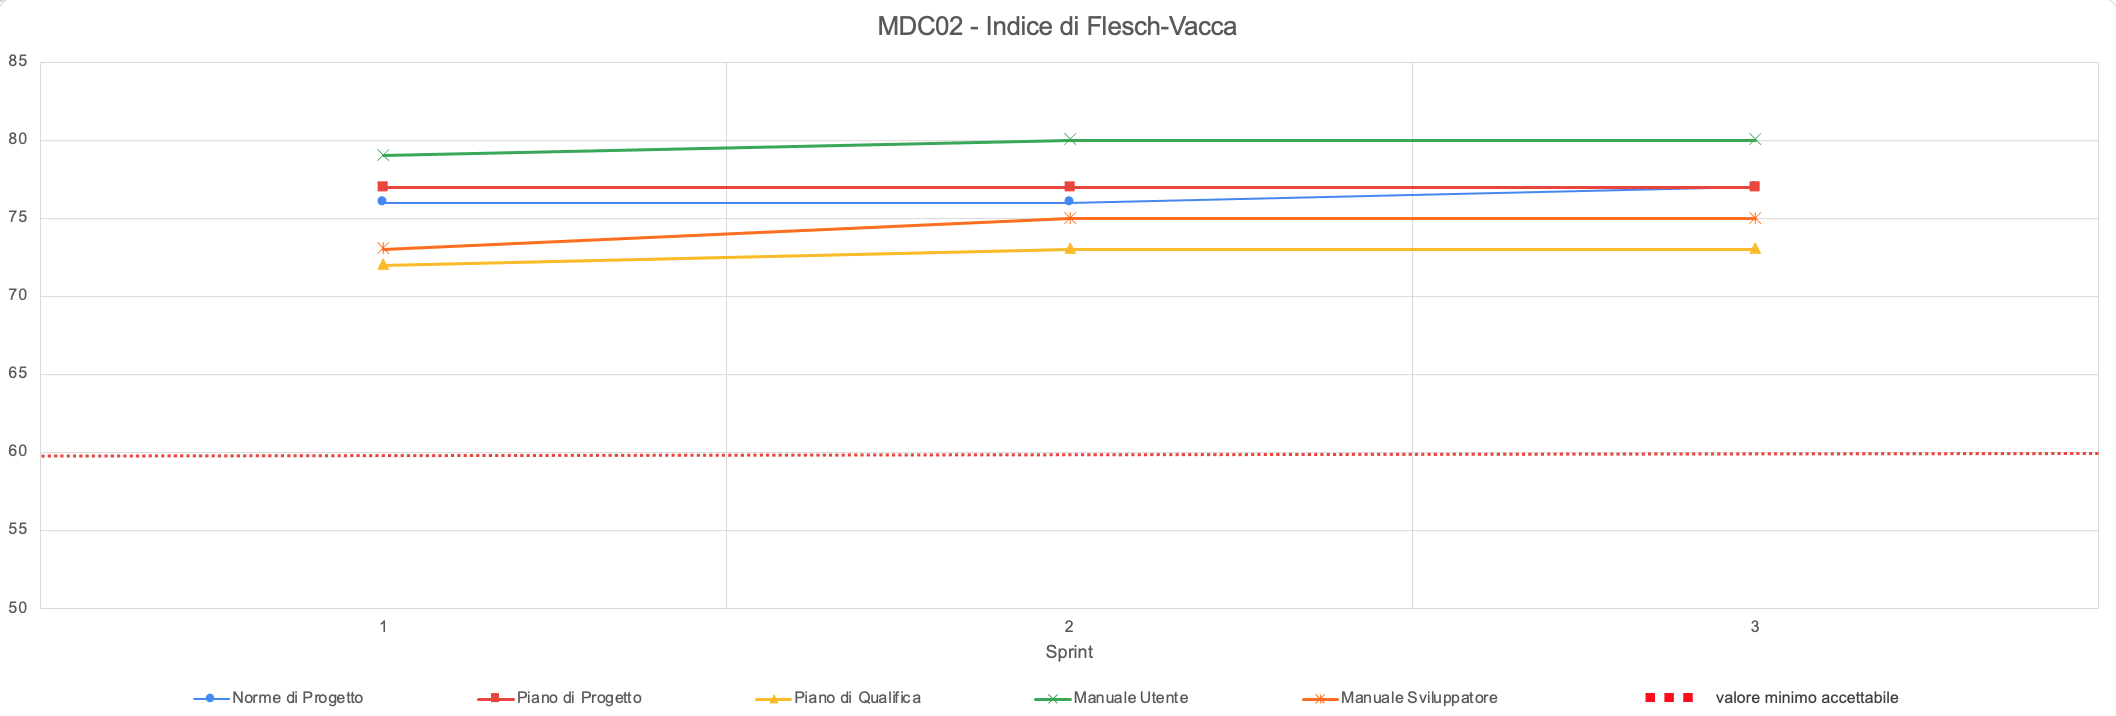
\includegraphics[scale = 0.6]{immagini/ImmRA/MDC02.png}
    \caption{Cruscotto MDC02, RA}
\end{figure}

\subsubsection*{MDC03 - correttezza ortografica}

\begin{figure}[H] 
    \centering
    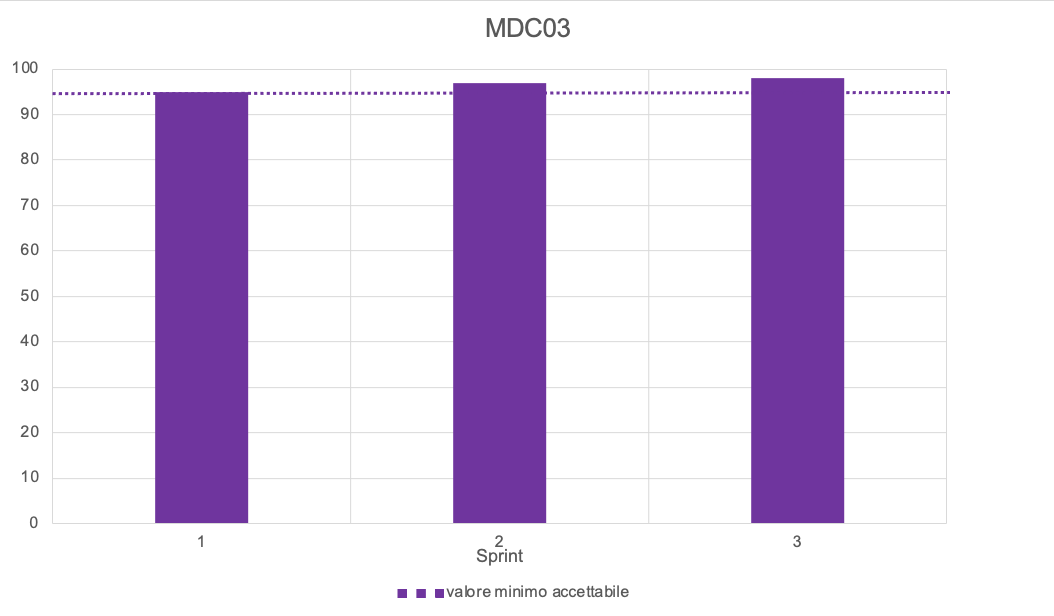
\includegraphics[scale = 0.8]{immagini/ImmRA/MDC03.png}
    \caption{Cruscotto MDC03, RA}
\end{figure}
\subsubsection{Cruscotto qualità del software}
Di seguito riportiamo i cruscotti dei valori riscontrati delle \glo{metriche} riguardanti il codice, descritte nel paragrafo \ref{QualitàSW} . In particolare, le metriche sono raggruppate in base al tipo, come normato nel documento \NdP{}.
\subsubsection*{MCD01 - percentuale degli errori gestiti}

\begin{figure}[H] 
    \centering
    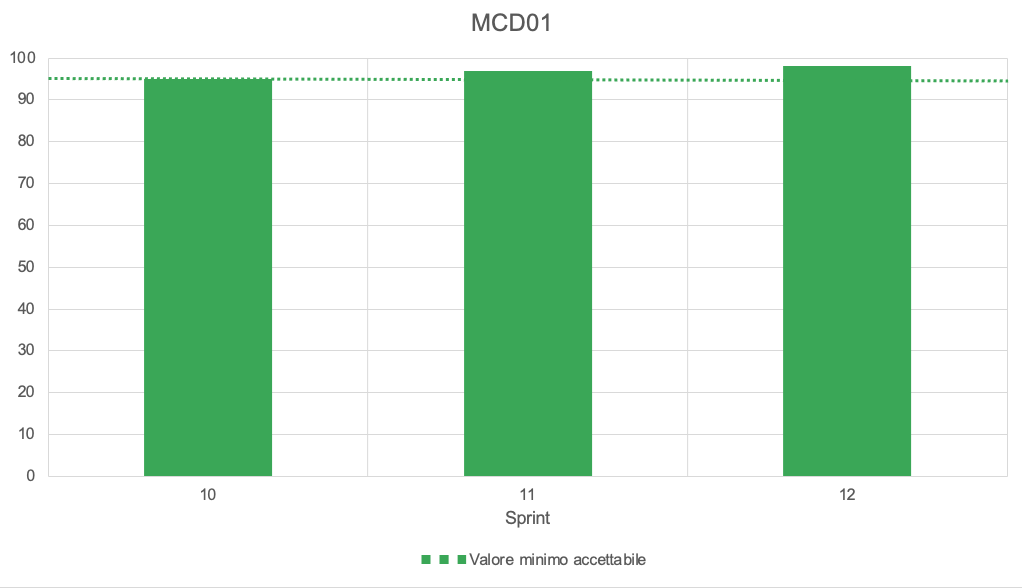
\includegraphics[scale = 0.65]{immagini/ImmRA/MCD01.png}
    \caption{Cruscotto MCD01, RA}
\end{figure}

\subsubsection*{MCD02 - complessità ciclomatica, MCD06 - lunghezza della riga di codice, MCD07 -brevità dei metodi }

\begin{figure}[H] 
    \centering
    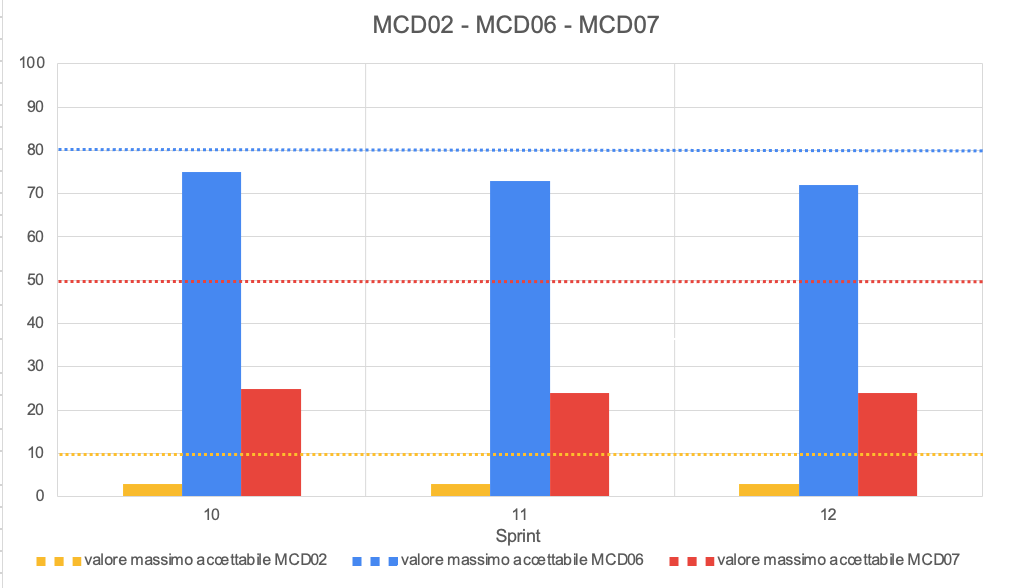
\includegraphics[scale = 0.8]{immagini/ImmRA/MCD020607.png}
    \caption{Cruscotto MCD02-MCD06-MCD07, RA}
\end{figure}

\subsubsection*{MCD03 - variabili non utilizzate, MCD04 - rapporto linee di codice e linee commentate }

\begin{figure}[H] 
    \centering
    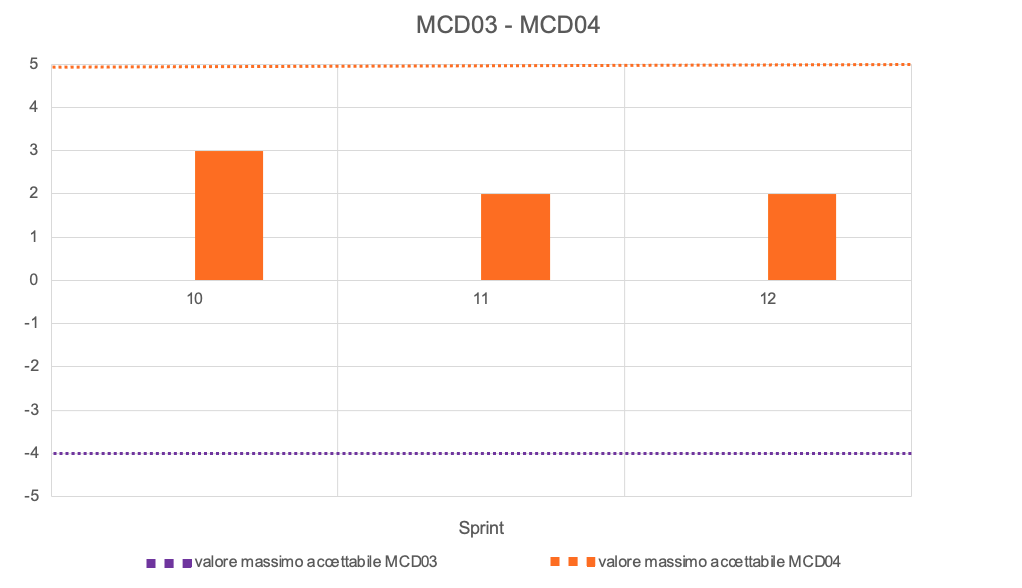
\includegraphics[scale = 0.8]{immagini/ImmRA/MCD0304.png}
    \caption{Cruscotto MCD03-MCD04, RA}
\end{figure}


\subsubsection*{MCD05 - code coverage }

\begin{figure}[H] 
    \centering
    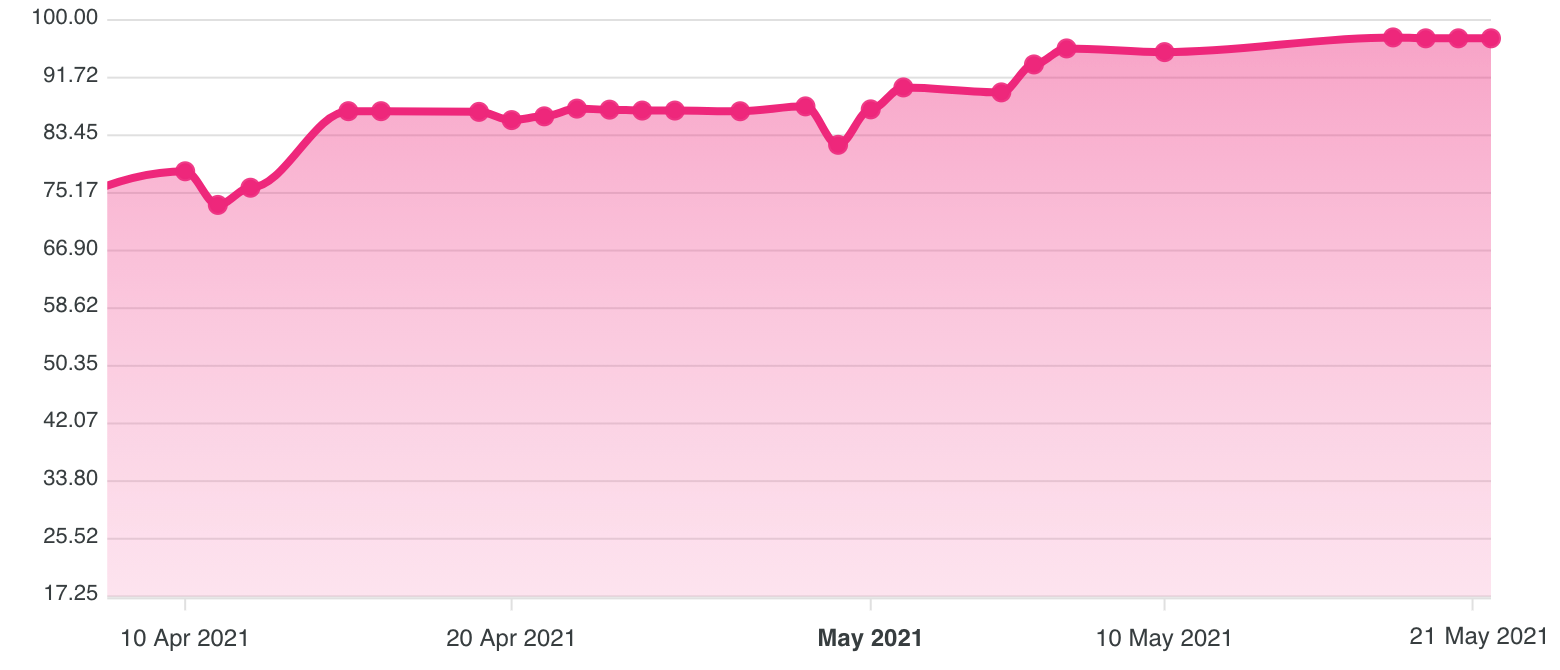
\includegraphics[scale = 1]{immagini/ImmRA/MCD05.png}
    \caption{Cruscotto MCD05, RA}
\end{figure}


\subsubsection*{MPR03 - soddisfazione requisiti obbligatori, MPR04 - soddisfazione requisiti opzionali }

\begin{figure}[H] 
    \centering
    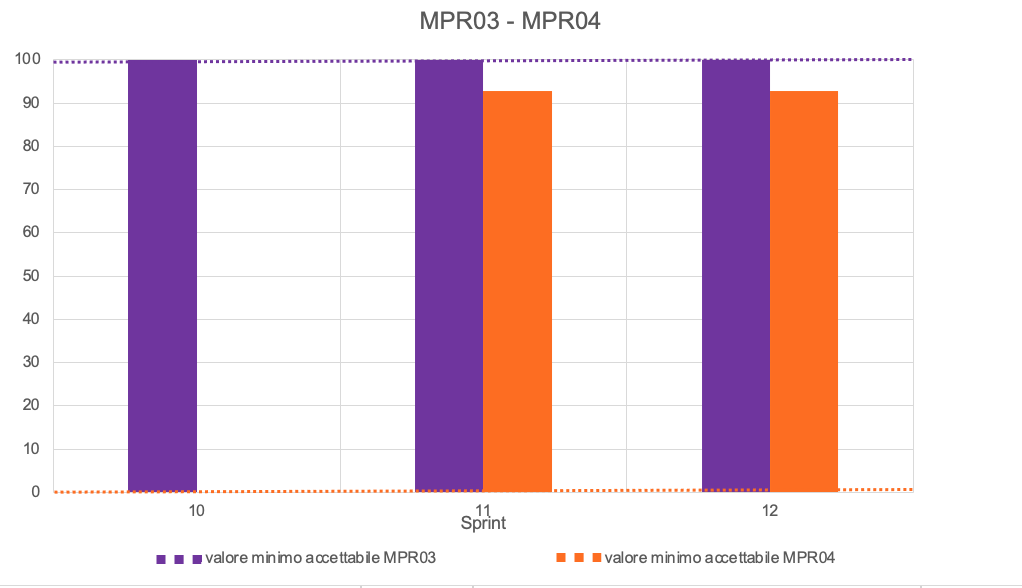
\includegraphics[scale = 0.8]{immagini/ImmRA/MPR0304.png}
    \caption{Cruscotto MPR03-MPR04, RA}
\end{figure}

\subsubsection*{MVR01 - percentuale malfunzionamenti test, MVR02 - comprensibilità delle funzionalità offerte, MVR04 -percentuale test passati, MVR05 -percentuale test falliti }

\begin{figure}[H] 
    \centering
    \includegraphics[scale = 0.5]{immagini/ImmRA/Mvr01020405.png}
    \caption{Cruscotto MVR01-MVR02-MVR04 - MVR05 RA}
\end{figure}

\subsubsection*{MVR03 - facilità di apprendimento e di utilizzo del prodotto}

\begin{figure}[H] 
    \centering
    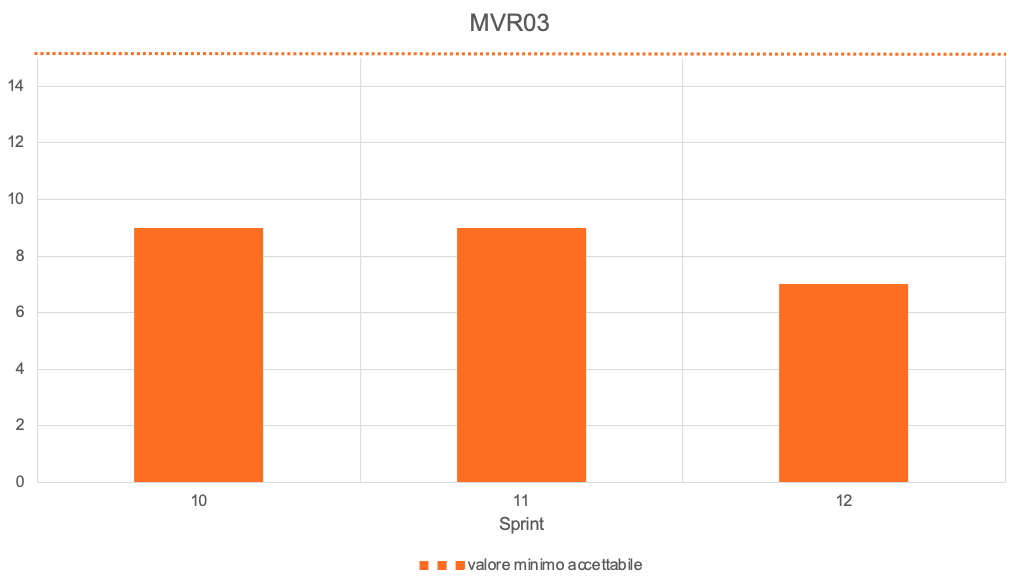
\includegraphics[scale = 0.7]{immagini/ImmRA/MVR03.png}
    \caption{Cruscotto MVR03, RA}
\end{figure}
